\clearpage
%//==============================--@--==============================//%
\subsection[3.6 Congestion control]{\hspace*{0.075 em}\raisebox{0.2 em}{$\pmb{\drsh}$} Congestion control}
\label{subsec:congestion-control}

\subsubsection[3.6.1 Approaches to Congestion Control]{$\pmb{\rightarrow}$ Approaches to Congestion Control}

At the highest level, we can distinguish among congestion-control approaches by whether the network layer provides explicit assistance to the transport layer for congestion-control purposes:

\begin{itemize}
    \item \textbf{Network-assisted congestion control:} In this approach, the network layer provides explicit feedback to the transport layer about the presence of congestion. The transport layer then adjusts its sending rate accordingly. Examples of this approach include ATM's ABR (Available Bit Rate) service and Frame Relay's BECN (Backward Explicit Congestion Notification) mechanism.
    
    \item \textbf{End-to-end congestion control:} In this approach, the network layer does not provide explicit feedback to the transport layer. Instead, the transport layer uses implicit feedback, typically from dropped packets or increased end-to-end delay, to infer the presence of congestion. The transport layer then adjusts its sending rate accordingly. The congestion-control mechanism used by TCP is an example of end-to-end congestion control.
\end{itemize}

\noindent Regardless of the approach taken, most congestion-control algorithms have the following objectives:

\begin{itemize}
    \item \textbf{Maximize network utilization:} The algorithm should aim to make the best use of available network resources, ensuring that network capacity is fully utilized whenever possible.
    
    \item \textbf{Fairness:} The algorithm should allocate resources fairly among competing flows, preventing any one flow from monopolizing the network.
    
    \item \textbf{Stability:} The algorithm should be able to react to changes in network conditions and maintain stable performance, avoiding oscillations in throughput or other undesirable behavior.
\end{itemize}

\subsubsection[3.6.2 Overview TCP]{$\pmb{\rightarrow}$ Overview TCP}

\noindent TCP sender limits its send rate using a congestion window (\texttt{cwnd}), which constrains the amount of unacknowledged data in the network. TCP detects congestion through loss events, either timeouts or three duplicate ACKs. In a congestion-free network, acknowledgments indicate successful data delivery, allowing the sender to increase \texttt{cwnd} and its send rate. TCP is self-clocking since it adjusts its congestion window size based on the rate of incoming acknowledgments:
$$
    \boxed{\texttt{LastByteSent} - \texttt{LastByteAcked} \leq \min\{\texttt{cwnd}, \texttt{rcvwnd}\}}
$$

\begin{enumerate}
    \item A lost segment implies congestion, and the sender should decrease its rate (by decreasing \texttt{cwnd}).
    \item An acknowledged segment indicates the network is delivering data, so the sender can increase its rate.
    \item \textbf{Bandwidth probing}: TCP increases its rate until a loss event occurs, then decreases the rate and probes again.
\end{enumerate}


\subsubsection[3.6.3 Classic TCP congestion control]{$\pmb{\rightarrow}$ Classic TCP congestion control}

\noindent \textbf{(1) Slow Start:}
\begin{itemize}[noitemsep, nolistsep]
    \item Initial \texttt{cwnd} is 1 MSS.
    \item Sender doubles sending rate every RTT.
    \item Exponential growth ends in three cases:
    \begin{itemize}[noitemsep, nolistsep]
        \item Timeout event: sets \texttt{cwnd} to 1 and \texttt{ssthresh} to \texttt{cwnd}/2 and starts slow start anew.
        \item \texttt{cwnd} equals \texttt{ssthresh}: transitions into congestion avoidance mode.
        \item Three duplicate ACKs: fast retransmit and enters fast recovery state.
    \end{itemize}
\end{itemize}

\vspace{0.5em}
\noindent \textbf{(2) Congestion Avoidance:}
\begin{itemize}[noitemsep, nolistsep]
    \item \texttt{cwnd} is approximately half its previous value.
    \item Increases \texttt{cwnd} by 1 MSS every RTT: common approach is to increase \texttt{cwnd} by MSS/\texttt{cwnd} when a new acknowledgment arrives.
    \item Linear increase (1 MSS per RTT) ends in two cases:
    \begin{itemize}
        \item Timeout event: set \texttt{cwnd} to 1 MSS, update \texttt{ssthresh} to half the value of previous cwnd.
        \item Triple duplicate ACK event: halve \texttt{cwnd} value, update \texttt{ssthresh} to half the value of previous \texttt{cwnd}, and enter fast-recovery state.
    \end{itemize}
\end{itemize}

\vspace{0.25em}
\noindent \textbf{(3) Fast Recovery} {\footnotesize (``Fast recovery is a \underline{recommended, but not required}, component of TCP''\cite{Kurose2017})}
\begin{itemize}[noitemsep, nolistsep]
    \item In fast recovery, increase \texttt{cwnd} by 1 MSS for every duplicate ACK received for the missing segment.
    \item Upon receiving an ACK for the missing segment, enter the congestion-avoidance state and deflate \texttt{cwnd}.
    \item If a timeout event occurs, perform the same actions as in slow start and congestion avoidance:
    \begin{itemize}
        \item Set \texttt{cwnd} to 1 MSS.
        \item Set \texttt{ssthresh} to half the value of \texttt{cwnd} when the loss event occurred.
    \end{itemize}
    \item After the timeout event, transition to the slow-start state.
\end{itemize}

\begin{figure}[H]
    \centering
    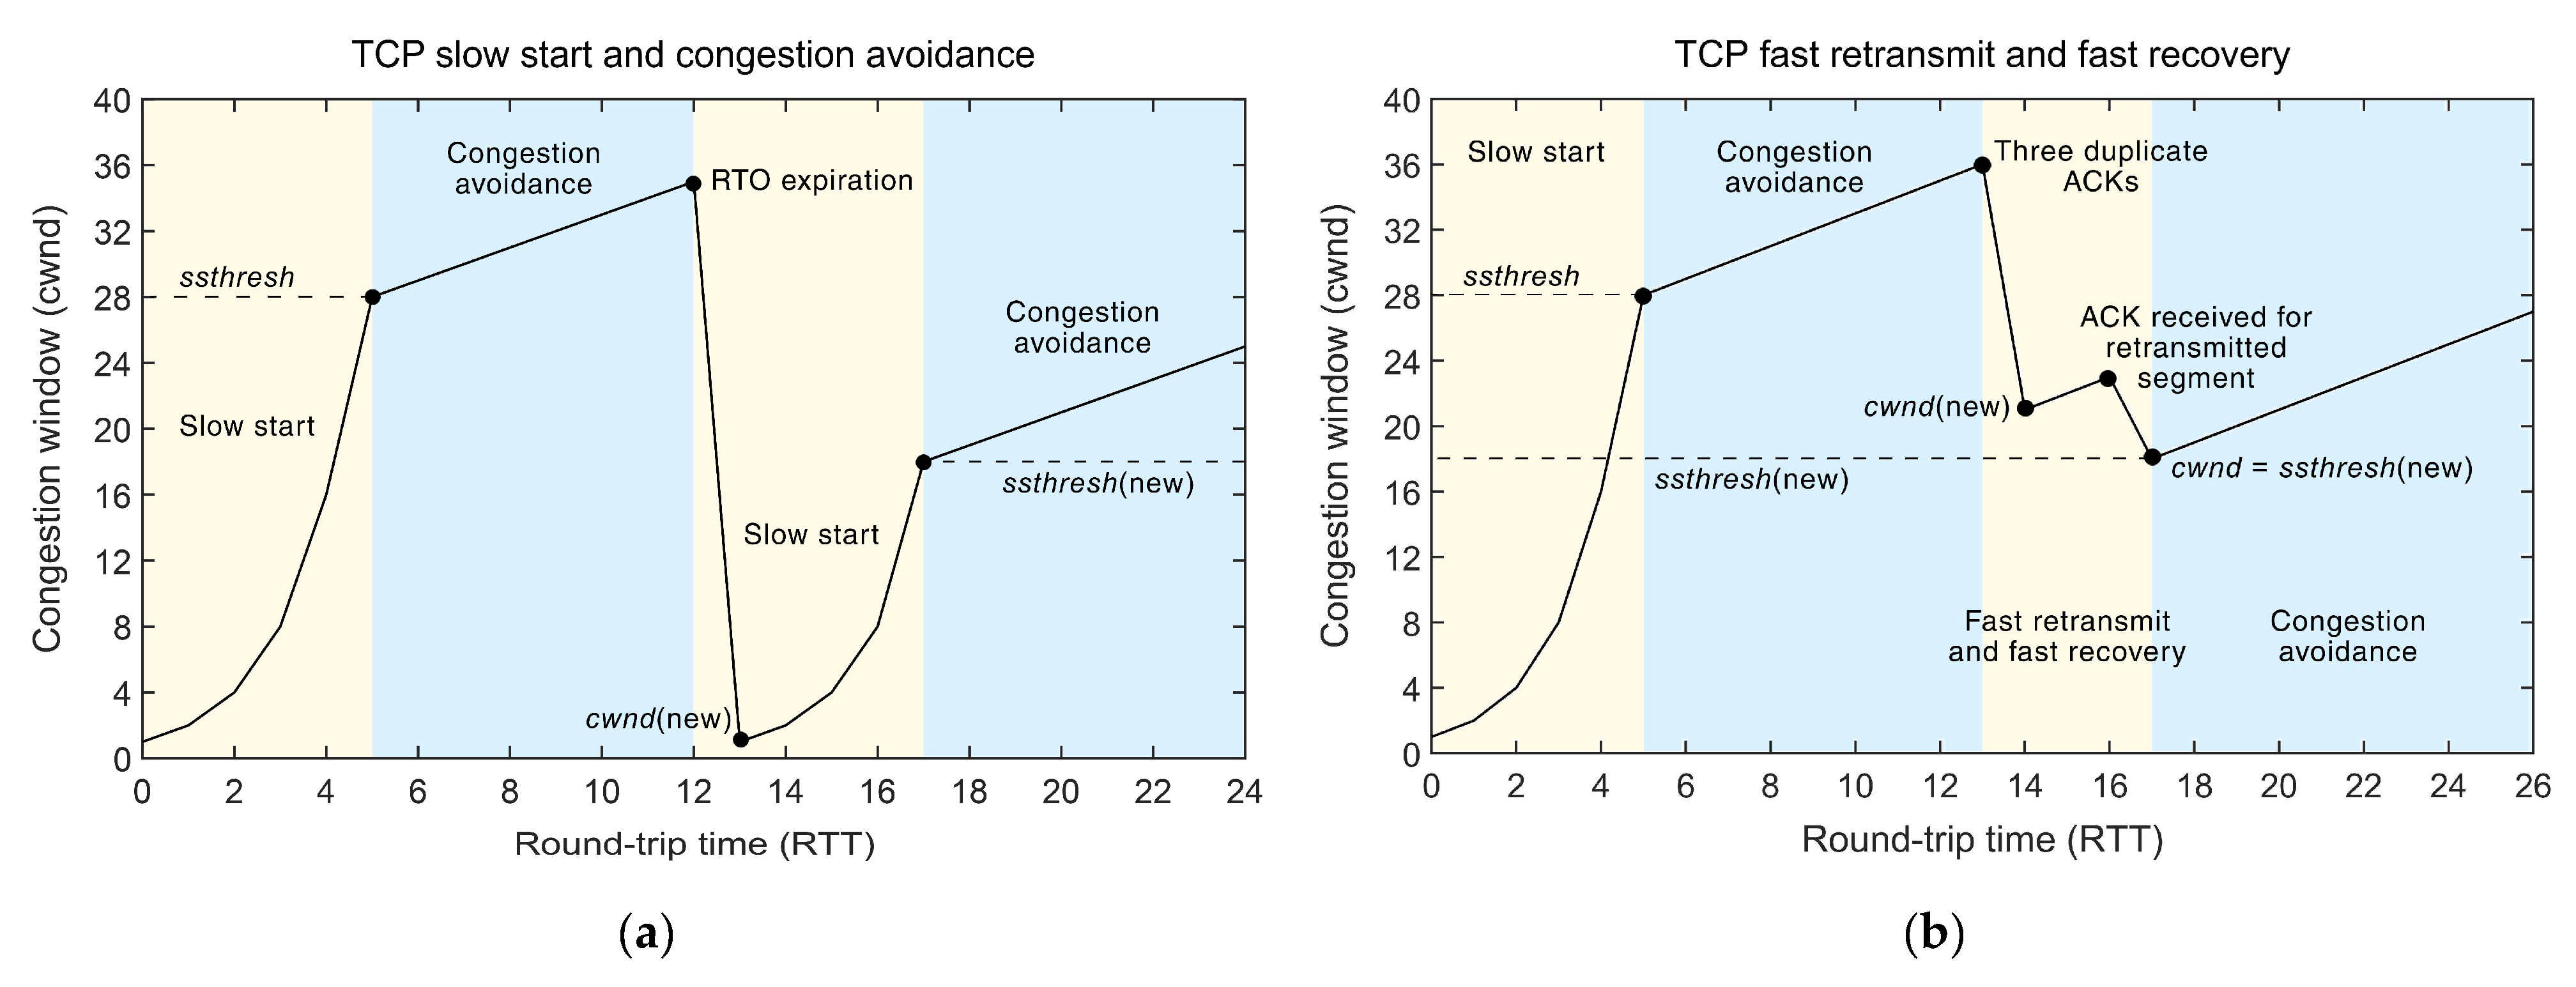
\includegraphics[width = 0.9\linewidth]{img/3/congestion-graphic.png}
    \caption{Standard working principles of the TCP CC mechanism related to the interdependence between \texttt{cwnd} and RTT for: (a) the TCP slow start and congestion avoidance mechanism; (b) the TCP fast retransmit and fast recovery mechanism. $[$Lorincz 2021$]$}
    \label{fig:congestion-graphic}
\end{figure}

\noindent ``For this reason, TCP congestion control is often referred to as an \textbf{additive-increase, multiplicative-decrease (AIMD)} form of congestion control.''\cite{Kurose2017}

\begin{figure}[H]
    \centering
    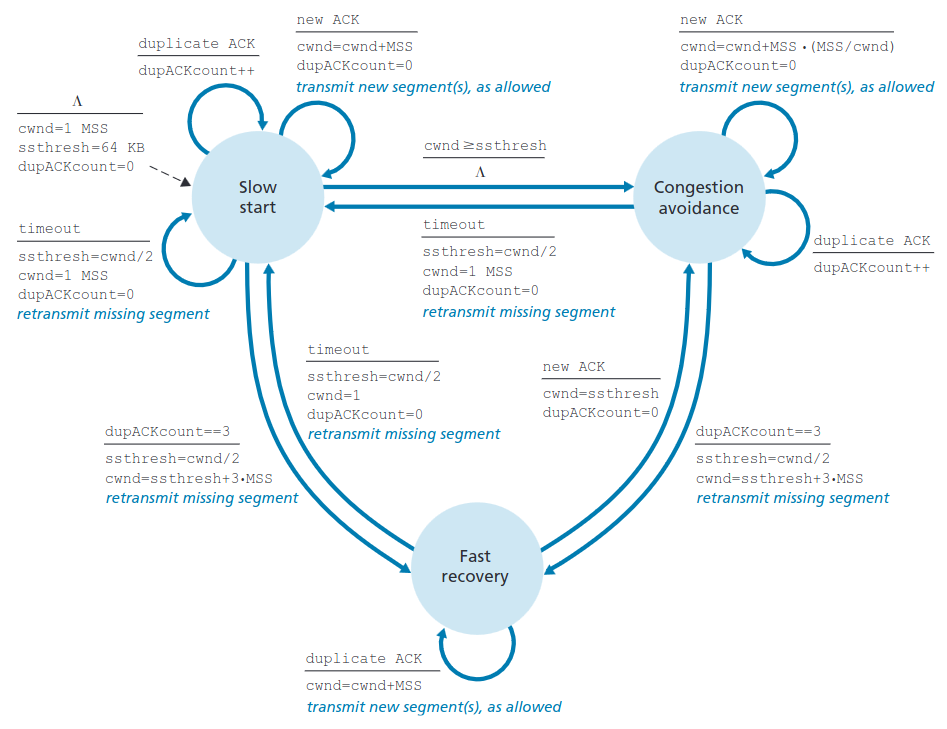
\includegraphics[width = 1\linewidth]{img/3/congestion-control-diagram.png}
    \caption{Diagrama de controlo de congestão TCP \cite{Kurose2017}}
    \label{fig:congestion-control-diagram}
\end{figure}

\paragraph[3.6.3.1 Nota histórica: TCP Tahoe \& TCP Reno]{$\pmb{\star}$ Nota histórica: TCP Tahoe \& TCP Reno}\mbox{}

\begin{figure}[ht]
    \centering
    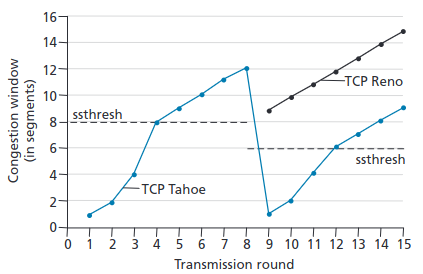
\includegraphics[width = 0.65\linewidth]{img/3/reno-tahoe.png}
    \caption{``Evolution of TCP’s congestion window (Tahoe and Reno)''\cite{Kurose2017}}
    \label{fig:tahoe-reno}
\end{figure}

\vspace{-1em}
\begin{quote}
    ``Fast recovery is a recommended, but not required, component of TCP $[$RFC 5681$]$. It is interesting that an early version of TCP, known as TCP Tahoe, unconditionally cut its congestion window to 1 MSS and entered the slow-start phase after either a timeout-indicated or triple-duplicate-ACK-indicated loss event. The newer version of TCP, TCP Reno, incorporated fast recovery.''\cite{Kurose2017}
\end{quote}

\newpage
\subsubsection[3.6.4 Extensions and Alternatives to TCP]{$\rightarrow$ Extensions and Alternatives to TCP}

\begin{itemize}
    \item \textbf{RED (Random Early Discard):} An active queue management strategy that randomly drops packets before the buffer is full, encouraging sources to reduce sending rates and preventing global synchronization of flows.
    
    \item \textbf{ECN (Explicit Congestion Notification):} A mechanism allowing routers to signal congestion to end-points by setting a flag in the packet header, allowing end-points to adjust their sending rates without waiting for packet loss as a signal.
    
    \item \textbf{TCP Vegas:} A congestion control algorithm that detects congestion early by monitoring the difference between expected and actual throughput, adjusting sending rates to avoid oscillations and maintain steady performance.
    
    \item \textbf{TCP BBR (Bottleneck Bandwidth and Round-trip propagation time):} A congestion control algorithm using the bottleneck bandwidth and round-trip time to estimate available network capacity, achieving higher throughput and lower latency than traditional loss-based algorithms.
    
    \item \textbf{CUBIC TCP:} A congestion control algorithm using a cubic function for window growth, enabling faster recovery from congestion and better performance in high-bandwidth, high-latency networks.
    
    \item \textbf{QUIC (Quick UDP Internet Connections):} A transport layer protocol developed by Google using UDP, offering faster connection establishment, built-in encryption, and improved congestion control compared to TCP, resulting in better web performance over high-latency networks.
\end{itemize}

\subsubsection[3.6.5 Congestion control fairness]{$\rightarrow$ Congestion control fairness}

Fairness in congestion control refers to the equal distribution of available bandwidth among concurrent connections. Various factors can affect the fairness of congestion control mechanisms:

\begin{itemize}
    \item \textbf{TCP's AIMD algorithm:} For TCP's AIMD algorithm, it converges to provide an equal share of a bottleneck link's bandwidth among competing TCP connections, as demonstrated by Chiu 1989. This algorithm allows TCP connections to adjust their transmission rates based on network congestion and fairly share the available bandwidth.
    
    \item \textbf{Varying RTTs:} Multiple connections sharing a common bottleneck with varying RTTs can lead to unequal bandwidth allocation. Connections with smaller RTTs can grab available bandwidth more quickly, resulting in higher throughput than connections with larger RTTs.
    
    \item \textbf{UDP vs. TCP:} Many multimedia applications often run over UDP to avoid TCP's rate throttling, leading to a potentially unfair distribution of resources. UDP sources can maintain constant transmission rates and occasionally lose packets, while TCP sources reduce their rates during congestion. As a result, UDP sources can crowd out TCP traffic, causing fairness concerns.
    
    \item \textbf{Real-world scenarios:} In real-world situations, the ideal conditions such as only TCP connections traversing the bottleneck link, connections having the same RTT value, and only a single TCP connection being associated with a host-destination pair are rarely met. As a result, these factors can lead to unequal bandwidth allocation among different connections in client-server applications.
\end{itemize}

%//==============================--@--==============================//%